\documentclass[11pt]{article}
\usepackage{graphicx}
\usepackage{amsthm}
\usepackage{latexsym}
\usepackage{amssymb}
\usepackage{amsmath}
\usepackage{listings}
\usepackage[usenames]{color}
\lstset{language=Java}
\usepackage{colortbl}
\definecolor{CommentColor}{rgb}{0,0.45,0.08}
\lstset{
    basicstyle=\ttfamily\small,
    keywordstyle=\color{blue},
    commentstyle=\color{CommentColor},
    tabsize=4
}
\newtheorem{theorem}{}
\newcommand{\ra}{\Rightarrow}
\renewcommand{\iff}{\Leftrightarrow}
\newcommand{\bt}{\textbf{T}}
\newcommand{\vc}[1]{\mathbf{#1}}
\newcommand{\dotp}[2]{\vc{#1} \cdot \vc{#2}}
\newcommand{\A}{$\mathcal{A}$\;}

% ********************************************
% ********** Hogwarts.sty ****************
\RequirePackage[garamond]{mathdesign} % The font used by JK Rowling's books
\RequirePackage[small,euler-digits]{eulervm} % Snape's favorite font
\RequirePackage{pifont} % Ron loves dingbats, see "psnfss2e.pdf"
\linespread{1.05} % make the typography more open, as Harry prefers
\renewcommand{\boldsymbol}[1]{\mathbold{#1}} % Dumbledore prefers bold characters to be set in eulervm
% ********************************************

\bigskip
\author{Priyananda Shenoy (shenoy@cs.wisc.edu)}
\title{	CS 540 Fall 2008 Homework 5}
\setlength{\parindent}{0in}

\begin{document}
\maketitle
\begin{center}
	Late Days used: \underline{0}
\end{center}

\newpage

\renewcommand{\labelenumi}{[\alph{enumi}]}

1.
\begin{enumerate}
	\item
	\begin{align*}
		P(Y|X) &= \frac{P(Y,X)}{P(X)} \\
			&= \frac{P(X,Y,Z) + P(X,Y,\lnot Z)}{P(X,Y,Z) + P(X,\lnot Y,Z) + P(X,Y, \lnot Z) + P(X,\lnot Y, \lnot Z)} \\
			&= \frac{0.70 + 0.015}{0.70 + 0.015 + 0.10 + 0.02} \\
			&= \mathbf{0.8563}
	\end{align*}
	
	\item
	\begin{align*}
		P(Y|X,Z) &= \frac{P(X,Y,Z)}{P(X,Z)} \\
			&= \frac{P(X,Y,Z)}{P(X,Y,Z) + P(X,\lnot Y,Z)} \\
			&= \frac{0.70}{0.70 + 0.10} \\
			&= \mathbf{0.875}
	\end{align*}
	
	\item
	\begin{align*}
		P(Y) &= P(X,Y,Z) + P(\lnot X,Y,Z) + P(X,Y,\lnot Z) + P(\lnot X, Y, \lnot Z) \\
			&= 0.70 + 0.015 + 0.08 + 0.01 \\
			&= \mathbf{0.805}
	\end{align*}
	
	\item
	\begin{align*}
		P(X,Z) &= P(X,Y,Z) + P(X,\lnot Y,Z) \\
			&= 0.70 + 0.10 \\
			&= \mathbf{0.80}
	\end{align*}
	
	\item If X and Z are independent, then the following should hold
	\[ P(X,Z) = P(X)P(Z). \]
	We can calculate P(X) and P(Z) as follows:
	\begin{align*}
		P(X) &= P(X,Y,Z) + P(X,\lnot Y,Z) + P(X,Y,\lnot Z) + P(X,\lnot Y,\lnot Z) \\
				 &= 0.70 + 0.015 + 0.10 + 0.02 = \mathbf{0.835} \\
		P(Z) &= P(X,Y,Z) + P(\lnot X,Y,Z) + P(X,\lnot Y,Z) + P(\lnot X,\lnot Y,Z) \\
				 &= 0.70 + 0.08 + 0.10 + 0.07  = \mathbf{0.95}\\
		P(X)P(Z) &= (0.835)(0.95) = \mathbf{0.7933}
	\end{align*}
	Since $P(X,Z) \neq P(X)P(Z)$, X and Z are not independent.
\end{enumerate}

2. Let the boolean random variables $\{HW,HANDIN,TP\}$ be defined as:
		\begin{itemize}
			\item $HW = true$ iff Jack finished the HW.
			\item $HANDIN = true$ iff Jack handed in the HW.
			\item $TP = true$ if Jack tells the professor that he forgot to handin the HW.
		\end{itemize}
	We know the following probabilities:
	\begin{itemize}
		\item $P(TP|HW,\lnot HANDIN) = 0.01$.
		\item $P(TP|\lnot HW) = 0.5$.
		\item $P(HW) = 0.9$.
	\end{itemize}
	We can make a few simplifying assumptions. Since Jack may be a liar but not a cheat,
	we can take $P(HANDIN|\lnot HW) = 0$. People who did submit will of course not
	lie to the professor, so $P(TP|HANDIN) = 0$. We are interested in finding
	if Jack did complete his homework, i.e. $P(HW|TP)$.
	\begin{align*}
		P(HW|TP) &= \frac{P(TP|HW)P(HW)}{P(TP)} \text{By Bayes' Rule} \\
		P(TP) 	 &= P(TP,HW,HANDIN) + P(TP,HW,\lnot HANDIN) \\
						 &	+ P(TP,\lnot HW,HANDIN) + P(TP,\lnot HW,\lnot HANDIN) \\
						 &= 0 + 0.01 + 0 + 0.5 = 0.501 \\
		P(TP|HW) &= P(TP,HW) P(HW) \\
						 &= (P(TP,HW,HANDIN) + P(TP,HW,\lnot HANDIN))P(HW) \\
						 &= (0 + 0.01)(0.5) = 0.005 \\
		P(HW|TP) &= \frac{0.005 \cdot 0.5}{0.501} = \mathbf{0.0049}
	\end{align*}
	
	So Jack is telling the truth with $0.49 \%$ probability. He shouldn't get any points
	for this assignment.
	
3. We will precalculate the following priors:
	\begin{align*}
		P(B) &= P(B|A)P(A) + P(B|\lnot A)P(\lnot A) = (0.2)(0.8) + (0.9)(1-0.8) = 0.34\\
		P(D) &= P(D|A,B)P(A)P(B) + P(D|\lnot A,B)P(\lnot A)P(B) \\
				 &+ P(D|A,\lnot B)P(A)P(\lnot B) + P(D|\lnot A,\lnot B)P(\lnot A)P(\lnot B) \\
				 &= (0.85)(0.8)(0.34) + (0.25)(0.8)(0.66) + (0.15)(0.2)(0.34) + (0.05)(0.2)(0.66) \\
				 &= 0.38
	\end{align*}
\begin{enumerate}
	\item
	\begin{align*}
		P(E|B,C) &= \frac{P(E)P(B|E)P(C|E,B)}{P(B)P(C|B)} \text{By conditional chain rule}\\
		P(E) &= P(D)P(E|D) + P(\lnot D)P(E|\lnot D) \\
			&= (0.38)(0.6) + (0.62)(0.5) = 0.538 \\
		P(C|E,B) &= P(C|B) \text{since C and E are independent given B}\\
			&= 0.95 \\
		P(B|E) &= \frac{P(E|B)P(B)}{P(E)} = \frac{P(E|D)P(D|B)P(B)}{P(E)} \\
			&= \frac{P(E|D)(P(D|A,B) + P(D|\lnot A,B))P(B)}{P(E)} \\
			&= \frac{(0.6)(0.85 + 0.15)(0.34)}{0.538} = 0.3792 \\
		P(E|B,C) &= \frac{(0.538)(0.3792)(0.95)}{(0.34)(0.95)} = \mathbf{0.6}
	\end{align*}
	
	\item
	\begin{align*}
		P(D|E,A) &= \frac{ P(D) P(A|D) P(E|D) }{ P(A) P(E|A)} \text{By conditional chain rule} \\
		P(E|A) &= P(E|D)P(D|A) \\
				&= P(E|D)(P(D|A,B)P(B|A) + P(D|A,\lnot B)P(\lnot|A)) \\
				&= (0.6)((0.85)(0.2) + (0.25)(0.9)) \\
				&= 0.237\\
		P(A|D) &= \frac{P(D|A)P(A)}{P(D)} \\
				&= \frac{ ((0.85)(0.2) + (0.25)(0.9))(0.8) }{0.38} \\
				&= 0.8316\\
		P(D|E,A) &= \frac{(0.38)(0.8316)(0.60)}{(0.8)(0.237)} = \mathbf{1}
	\end{align*}
\end{enumerate}

4.
\begin{enumerate}
	\item The Markov model has three states $\{S,A,NA\}$. S corresponds to a start state, A
	corresponds to the lever being `on', and NA corresponds to the lever being 'off'.
	The state transition matrix \A is given as follows:
	\[ \mathcal{A} = \left( \begin{array}{cccc}
			 		& S & A 	& NA 	\\
			S:  & 0 & 0.5 & 0.5 \\
			A:  & 0 & 0.7 & 0.3 \\
			NA: & 0 & 0.3 & 0.7 \\
		 \end{array} \right)
	\]
	The initial state vector is given by $\pi = ( \begin{array}{ccc} 1.0 & 0 & 0 \end{array} )$.
	
	\begin{center} 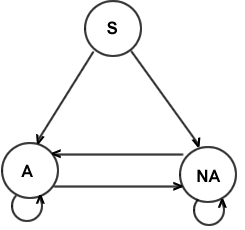
\includegraphics[width=150px,height=150px]{4a.png} \end{center}
	
	\item The Markov model now has five states $\{S,AC,ANC,NAC,NANC\}$, where S is the start
	state, `AC' corresponds to both almond and cononut levers being on, `ANC' corresponds to
	almond lever being on and cocunut lever being off, `NAC' corresponds to almond lever
	being off and coconut lever of, `NANC' corresponds to all levers being off. The state
	transition matrix is given by:
	\[ \mathcal{A} = \left( \begin{array}{rccccc}
			 		 & S & AC 	& ANC  & NAC  & NANC \\
			S:   & 0 & 0.25 & 0.25 & 0.25 & 0.25 \\
			AC:  & 0 & 0.49 & 0.21 & 0.21 & 0.09 \\
			ANC: & 0 & 0.21 & 0.49 & 0.09 & 0.21 \\
			NAC: & 0 & 0.21 & 0.09 & 0.49 & 0.21 \\
			NANC:& 0 & 0.09 & 0.21 & 0.21 & 0.49 \\
		 \end{array} \right)
	\]
	For the model to remain in the same state, neither of the levers must be changed which can
	happen with probability $(1-0.3)(1-0.3) = 0.49$. Similarly to go to a state where both the
	lever have changed, the probability is $(0.3)(0.3) = 0.09$. To go to a state where only one
	lever has changed, the probability is $(0.3)(1-0.3) = 0.21$.
	The initial state vector is given by $\pi = ( \begin{array}{ccccc} 1.0 & 0 & 0 & 0 & 0 \end{array} )$.
	
	\begin{center} 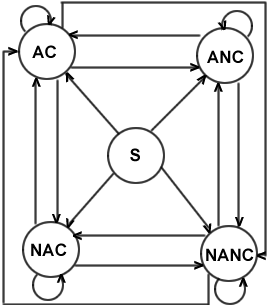
\includegraphics[width=170px,height=150px]{4b.png} \end{center}
	
	\item \begin{align*}
		&P(Plain,Almond,Almond,Almond+Coconut)\\
		&= P(NCNC|S) P(ANC|NCNC) P(ANC|ANC) P(AC|ANC) \\
		&= (0.25)(0.21)(0.49)(0.21) \\
		&= \mathbf{0.005402}
	\end{align*}
\end{enumerate}

5.
	\begin{enumerate}
	\item \textbf{Empty documents are classified on the basis of prior probabilities}
	\item For the given training set, the prior probabilities are given below:
	\begin{align*}
	P(English)  &= 0.272727 \\
	P(Spanish)  &= 0.389610 \\
	P(Japanese) &= 0.337662
	\end{align*}
	The conditional probabilities for each character given a languages is as follows:

	\begin{tabular}{|c|c|c|c|}
		\hline
			Char(c)	&$P(c|English)$&$P(c|Spanish)$&$P(c|Japanese)$\\
		\hline	
			a				&0.061609			&0.107405			&0.131701			\\
			b				&0.011893			&0.010668			&0.010015			\\
			c				&0.021727			&0.037540			&0.005156			\\
			d				&0.022358			&0.039021			&0.016358			\\
			e				&0.106133			&0.110281			&0.059925			\\
			f				&0.019941			&0.007105			&0.003374			\\
			g				&0.016178			&0.008199			&0.014792			\\
			h				&0.046502			&0.005366			&0.030935			\\
			i				&0.054742			&0.049088			&0.098364			\\
			j				&0.000824			&0.007147			&0.002186			\\
			k				&0.003955			&0.000300			&0.057037			\\
			l				&0.030269			&0.052350			&0.001026			\\
			m				&0.022166			&0.023868			&0.040814			\\
			n				&0.057599			&0.054583			&0.056929			\\
			o				&0.065290			&0.072569			&0.091076			\\
			p				&0.016343			&0.023997			&0.000540			\\
			q				&0.000659			&0.007147			&0.000027			\\
			r				&0.050567			&0.060034			&0.041948			\\
			s				&0.063367			&0.065894			&0.043298			\\
			t				&0.083061			&0.034707			&0.058414			\\
			u				&0.025517			&0.034535			&0.070507			\\
			v				&0.009311			&0.005988			&0.000135			\\
			w				&0.015437			&0.000279			&0.020245			\\
			x				&0.001181			&0.002382			&0.000000			\\
			y				&0.013349			&0.007384			&0.014711			\\
			z				&0.000549			&0.003670			&0.007774			\\
			space	  &0.179471			&0.168491			&0.122712			\\
		\hline
	\end{tabular}
	
	\item For the given test set, the confusion matrix is
		given below
		
		\begin{tabular}{|c|c|c|c|}
		\hline
					          &English	&Spanish	&Japanese \\
		\hline
					English		&15				&0				&0				\\
					Spanish		&15				&30				&0				\\
					Japanese	&0				&0				&30				\\
		\hline
		\end{tabular}
	
	\item Nowhere in the conditional probability calculation is the position
		of a character important. The classifier only looks at relative
		frequencies of characters in a language, and is therefore independent
		of the ordering of the characters. Hence, our classifier would output
		the same value it used to before the letters were scrambled.
	
	\item All natural languages possess much more structure than what the
	naive classifier looks for. For example, the values of preceding character(s)
	often narrows down the probable value of the next character. This can
	be extended to arbitrarily large syntactic structures(words, phrases, sentences etc).
	In practice, the relative frequencies of digrams(groups of two characters)
	and trigrams(groups of three characters) are used for classification.
	
	Most languages also treat white space with much less importance than
	what the classifier does. For example, groups of adjacent white space
	can be counted only once to avoid giving too much importance to white space.
	
	\end{enumerate}

6.
\begin{lstlisting}[frame=single]
[shenoy@cs]$ forget --help
	forget(8) is a tool developed by Univ of Wisconsin,
	Madison. Using advanced techniques like Bayesian
	Indifference, Pedantically arbitrarily complicated
	(PAC) unlearning and Statistical Senility, forget
	forgets even the most memorable things.
	Report bugs to shenoy@cs.wisc.edu.

[shenoy@cs]$ forget todays-date

[shenoy@cs]$ date
	0:0:0 0:0:0 some day, some time zone

[shenoy@cs]$ su
	password:
	incorrect password

[shenoy@cs]$ forget root-password

[shenoy@cs]$ su

[root@cs]$ forget ex-girlfriend
	deleting 1038 pictures            [DONE]
	deleting 227 emails               [DONE]
	removing her from facebook profile[DONE]
	reactivating match.com profile    [DONE]	

[root@cs]$ forget pennstate-beating-badgers
	forgetting complete with 1 warning(s)
	warning: Reality not changed: we still lost.

[root@cs]$ forget cs540-hw5
	forgetting failed: cs540-hw5 marked as unforgettable.

[root@cs]$ forget everything
	Are you sure you want to forget everything[Y/n]:y

[?@?]$ ls
	huh?

[?@?]$ reboot
	huh?

[?@?]$ help
	huh?
\end{lstlisting}
\end{document}